\section{Latent propagators}
% Original presentation frame 10
\begin{frame}[t,shrink=5]{Attention  might not be  All You Need , but it is a powerful tool for sequence modeling}
\begin{columns}[T,onlytextwidth]
\begin{column}{0.49\textwidth}
\begin{block}{Attention mechanism}
Each lattice element has a token $h_j$. For the update at $i$:
\[q_i=W_Qh_i,\quad k_j=W_Kh_j,\quad v_j=W_Vh_j.\]
\scriptsize What the current element needs; how upstream element $j$ is matched; information that element $j$ can contribute.
\end{block}
\begin{alertblock}{Compare, normalize, then combine}
\[s_{ij}=\frac{q_i^\top k_j}{\sqrt{d_k}},\quad j\le i,\]
\[\alpha_{ij}=\operatorname{softmax}_{j\le i}(s_{ij}),\quad\sum_{j\le i}\alpha_{ij}=1,\]
\[c_i=\sum_{j\le i}\alpha_{ij}v_j.\]
\scriptsize Larger $\alpha_{ij}$ means a stronger contribution from element $j$.
\end{alertblock}

\end{column}
\begin{column}{0.49\textwidth}
\begin{center}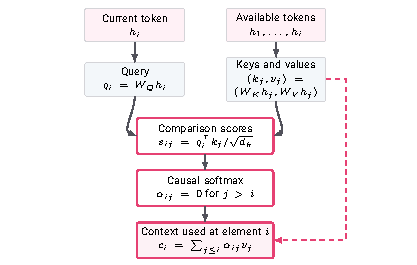
\includegraphics[width=\linewidth,height=42mm,keepaspectratio]{causal_attention_flow.pdf}\end{center}\begin{block}{Global causal attention}
Any $h_1,\ldots,h_i$ may contribute; downstream tokens are masked.
\par\smallskip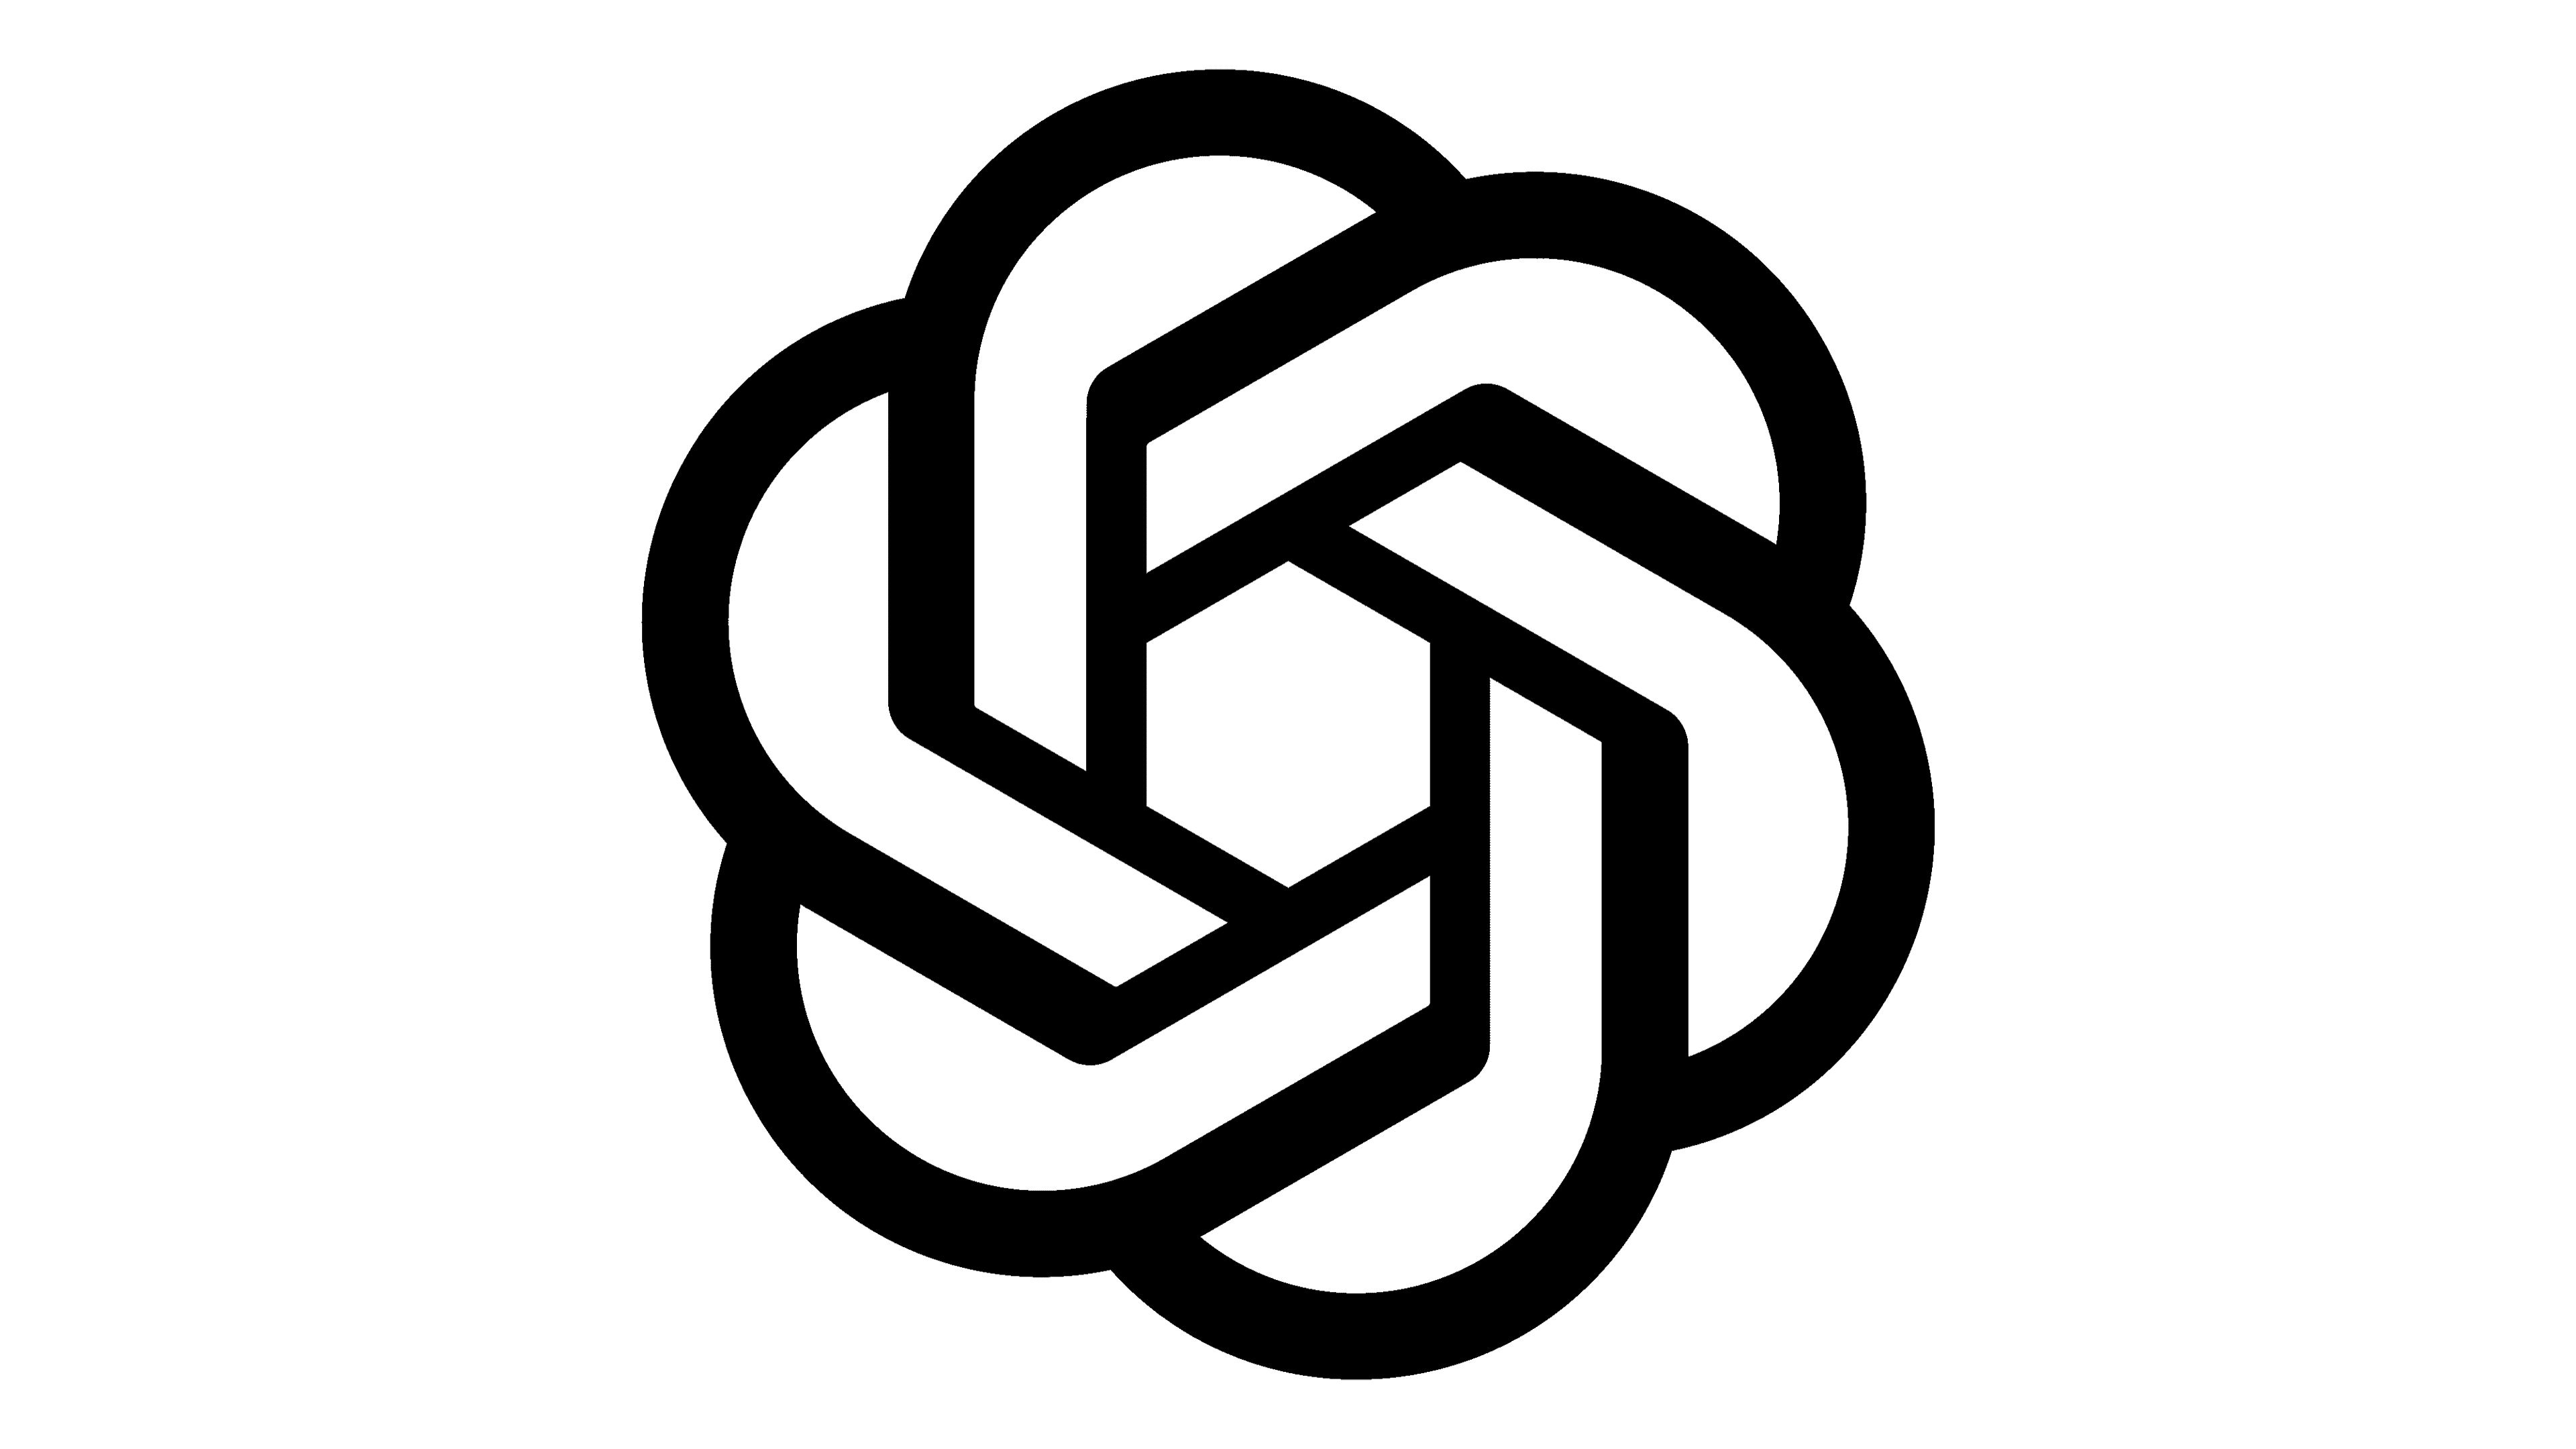
\includegraphics[width=14mm]{attention_illustration.png}
\end{block}

\end{column}
\end{columns}

\sources{Original Transformer formulation: \parencite{vaswani2017attention}.}

\end{frame}

% Original presentation frame 11
\begin{frame}[t,shrink=5]{Global causal attention respects lattice order but permits dense upstream mixing}
\begin{columns}[T,onlytextwidth]
\begin{column}{0.49\textwidth}
\begin{block}{Element-conditioned latent sequence}
\[z_{i+1}=z_i+\Delta z_i,\quad\Delta z_i=f_\theta(z_i,h_i,\mu).\]
Causal masking enforces upstream $\to$ downstream order, but token $i$ can directly aggregate all $j\le i$.
\end{block}
\begin{alertblock}{Selected endpoint checkpoint}
\[\epsilon_{\rm rel}=0.681,\quad\mathrm{SW}=0.087,\]\[\tau=18.74\ \mathrm{ms/sample}.\]
\end{alertblock}

\end{column}
\begin{column}{0.49\textwidth}
\begin{center}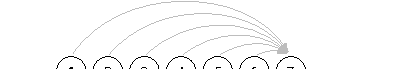
\includegraphics[width=\linewidth]{global_causal_attention_graph.pdf}\end{center}\begin{center}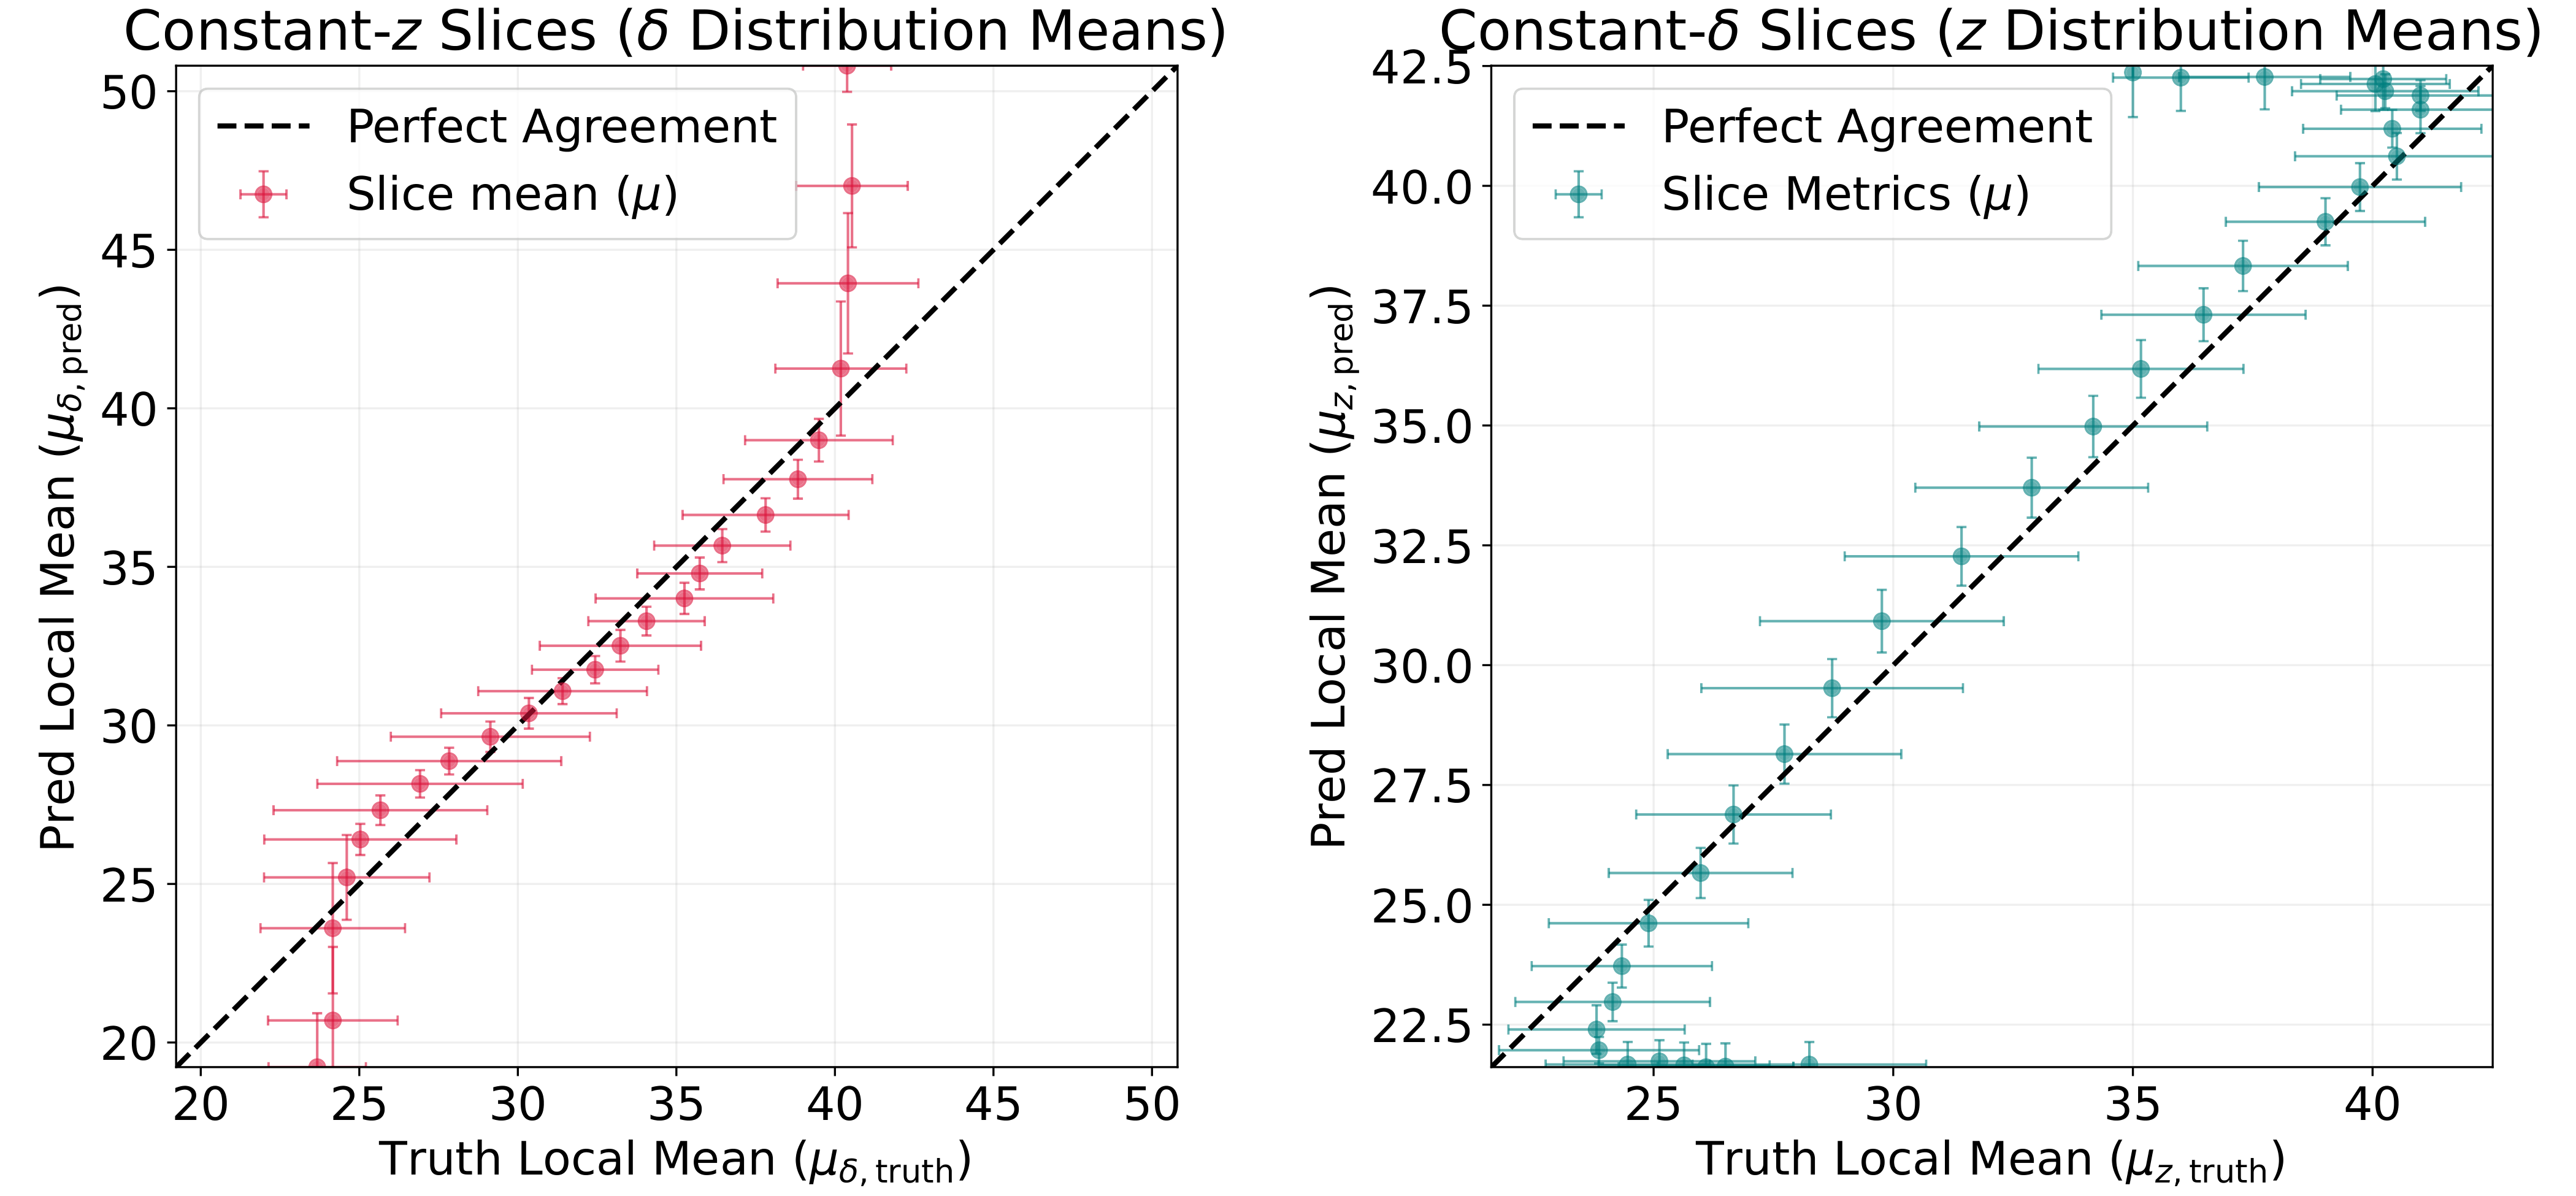
\includegraphics[width=\linewidth]{global_transformer_longitudinal_slices.png}\end{center}{\scriptsize Conditional-slice diagnostic: coherent longitudinal distortion is visible, but the figure does not prove global attention is its unique cause.\par}
\end{column}
\end{columns}

\sources{\parencite{vaswani2017attention,wang2026latent}.}

\end{frame}

% Original presentation frame 12
\begin{frame}[t,shrink=5]{Restricting direct attention support improves the endpoint task without changing the representation}
\begin{columns}[T,onlytextwidth]
\begin{column}{0.49\textwidth}
\begin{block}{Local causal support}
\[M_{ij}^{(w)}=\begin{cases}0,&0\le i-j\le w,\\-\infty,&\text{otherwise}.\end{cases}\]
Stacked layers still build longer-range dependence through repeated local composition.
\end{block}
\begin{alertblock}{Held-out endpoint change at $w=8$}
\[\epsilon_{\rm rel}:0.681\to0.534,\]\[\mathrm{SW}:0.087\to0.022.\]Only the admissible support of direct information transfer is changed.
\end{alertblock}

\end{column}
\begin{column}{0.49\textwidth}
\begin{center}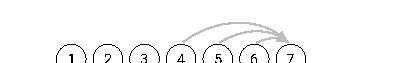
\includegraphics[width=\linewidth]{local_window_attention_graph.pdf}\end{center}\begin{center}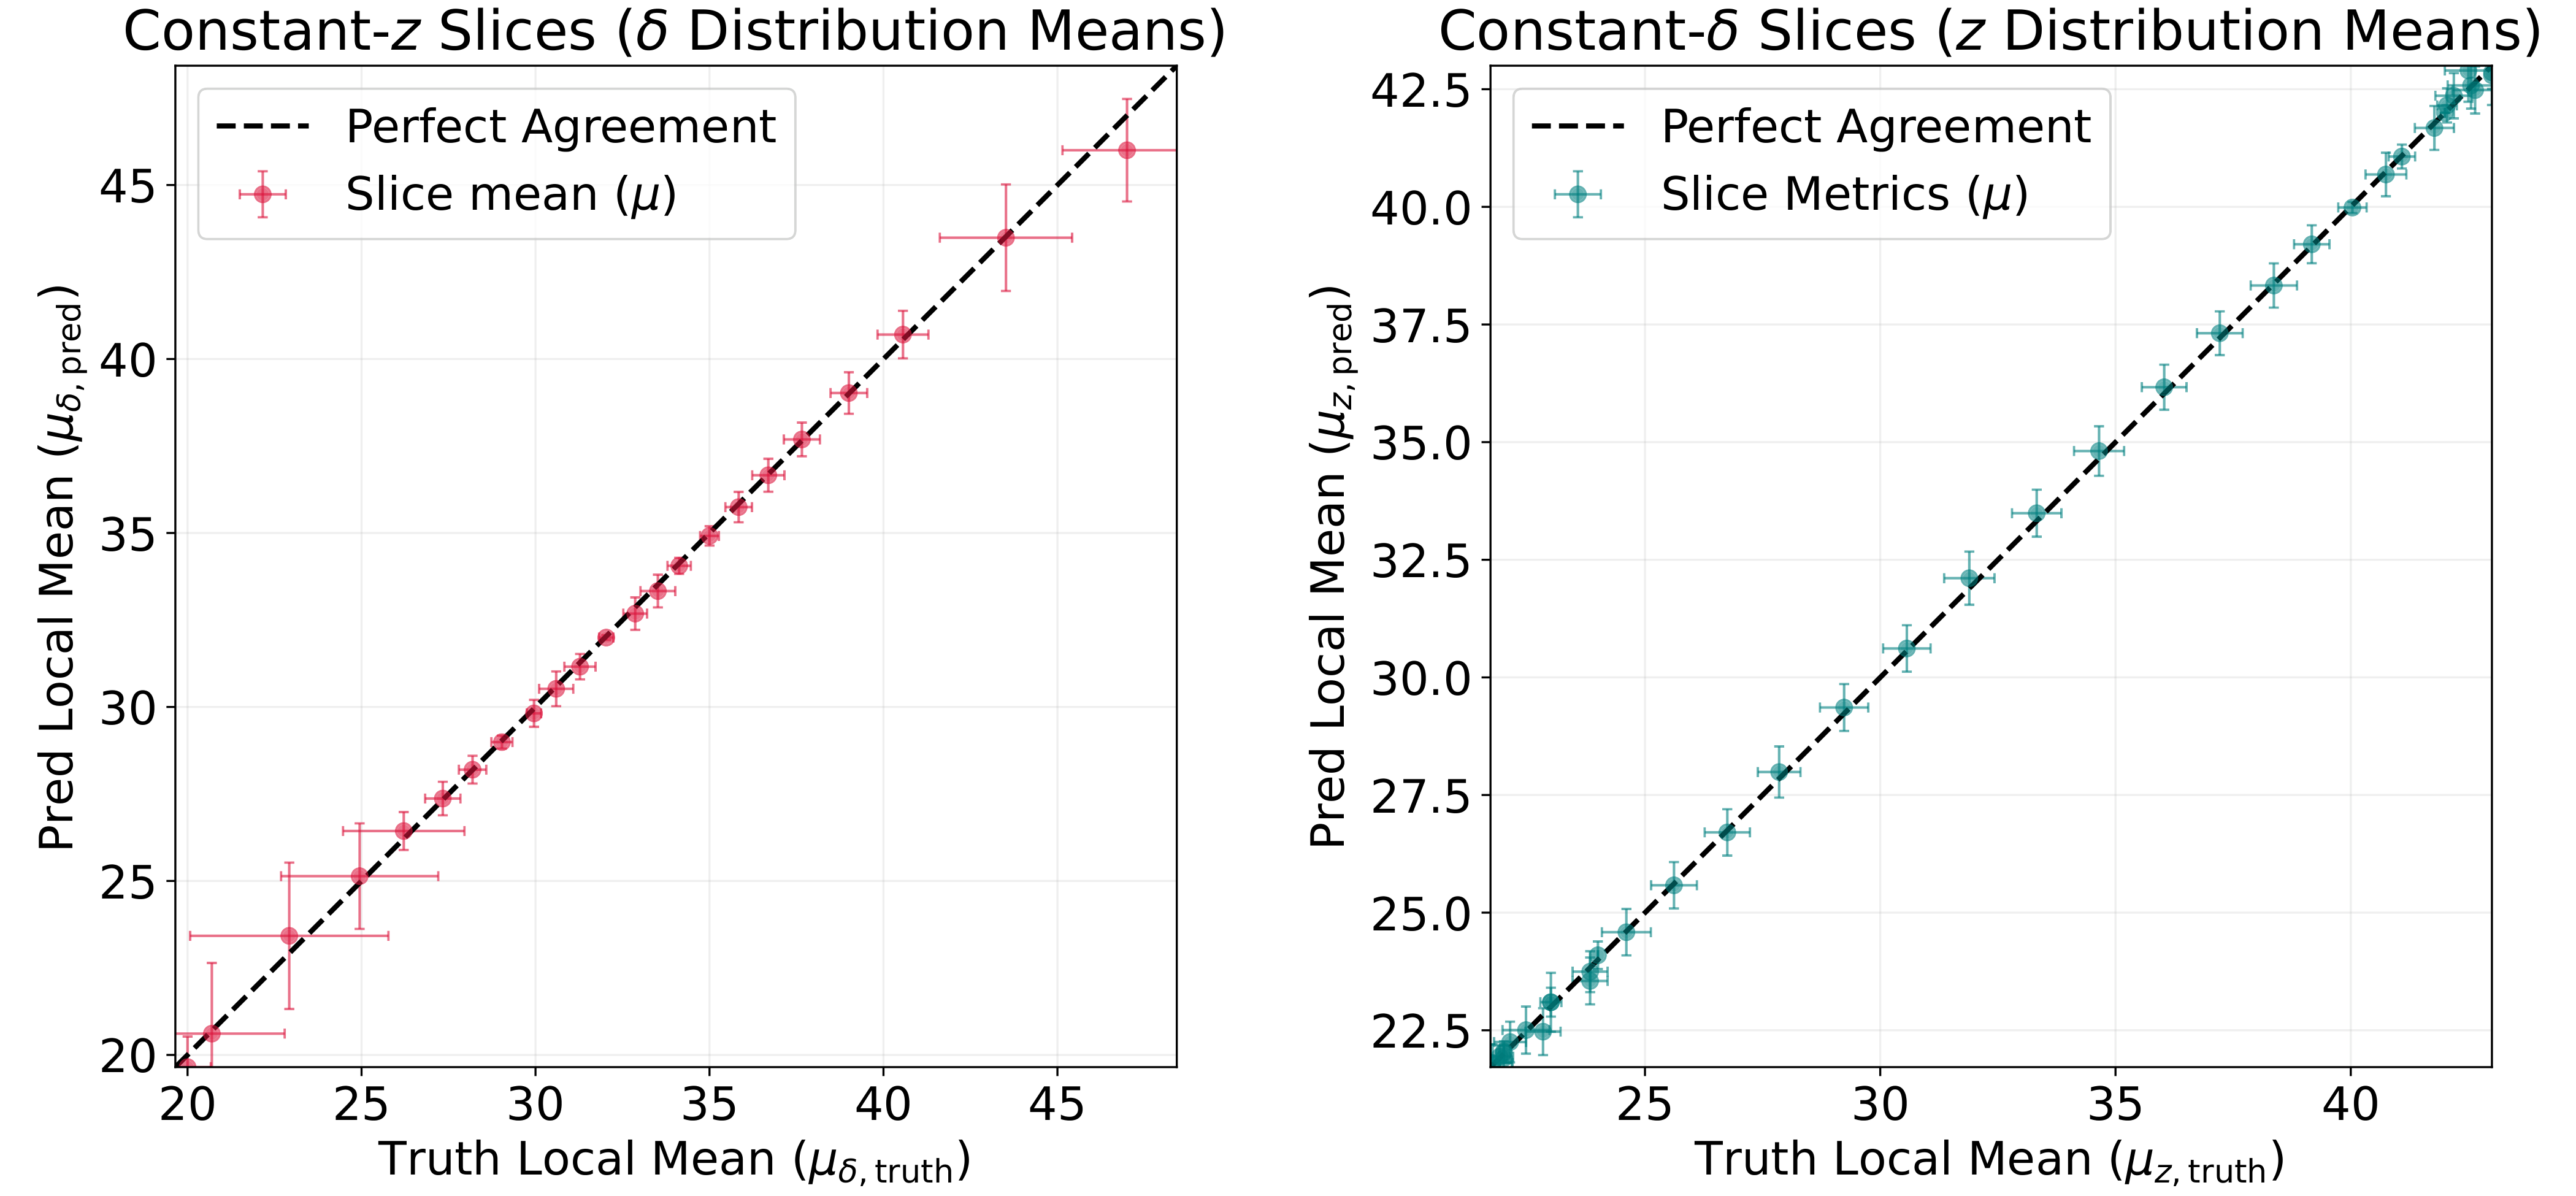
\includegraphics[width=\linewidth]{windowed_transformer_longitudinal_slices.png}\end{center}{\scriptsize Local-window Transformer conditional-slice result for the longitudinal $(\zeta,\delta)$ marginal.\par}
\end{column}
\end{columns}

\sources{\parencite{vaswani2017attention}.}

\end{frame}

% Original presentation frame 13
\begin{frame}[t,shrink=5]{Neural operators match the mathematical type of distribution evolution}
\begin{columns}[T,onlytextwidth]
\begin{column}{0.49\textwidth}
\begin{block}{Finite-dimensional network}
\[x\in\mathbb R^n\longmapsto y\in\mathbb R^m.\]The map is tied to finite dimensional vector representations of the data.
\end{block}
\begin{block}{Operator model}
\[a(\cdot)\longmapsto u(\cdot),\qquad\rho_{\rm in}\longmapsto\rho_{\rm out}.\]The object transformed is a field, profile or distribution.
\end{block}

\end{column}
\begin{column}{0.49\textwidth}
\begin{block}{Generic operator layer}
\[\begin{aligned}v_{\ell+1}(x)=\sigma\Bigl(&\underbrace{W_\ell v_\ell(x)}_{\text{local update}}\\&+\int_D\underbrace{\kappa_\theta(x,y;\mu)}_{\text{learned interaction kernel}}v_\ell(y)\,\mathrm d\nu(y)\Bigr).\end{aligned}\]
\end{block}
\begin{itemize}
\item The architecture chooses how to parameterize the kernel $\kappa_\theta$ and which points are allowed to interact.
\item FNO and GNO are two different kernel parameterizations of this same operator-learning idea.
\end{itemize}
\end{column}
\end{columns}

\sources{\parencite{kovachki2021fno,kovachki2023operators,li2020graph}.}

\end{frame}

% Original presentation frame 14
\begin{frame}[t,shrink=5]{FNO is a controlled longitudinal benchmark because wake response is already spectral}
\begin{columns}[T,onlytextwidth]
\begin{column}{0.49\textwidth}
\begin{block}{Physical and learned operators use the same representation}
\[V_{\rm ind}(z)=-\mathcal F^{-1}[Z_\parallel(\omega;\mu)\widehat\lambda(\omega)](z),\]
\[\mathcal K_\theta^{\rm FNO}v=\mathcal F^{-1}[R_\theta(k)\mathcal F(v)(k)].\]
\end{block}
\begin{block}{Benchmark scope}
2048 PyColleff samples, 2048 longitudinal grid points, 3 GeV ring, $Q=10^4$, three relaxation steps with $\alpha=0.7$. This is separate from the 6D HEB dataset.
\end{block}

\end{column}
\begin{column}{0.49\textwidth}
\begin{center}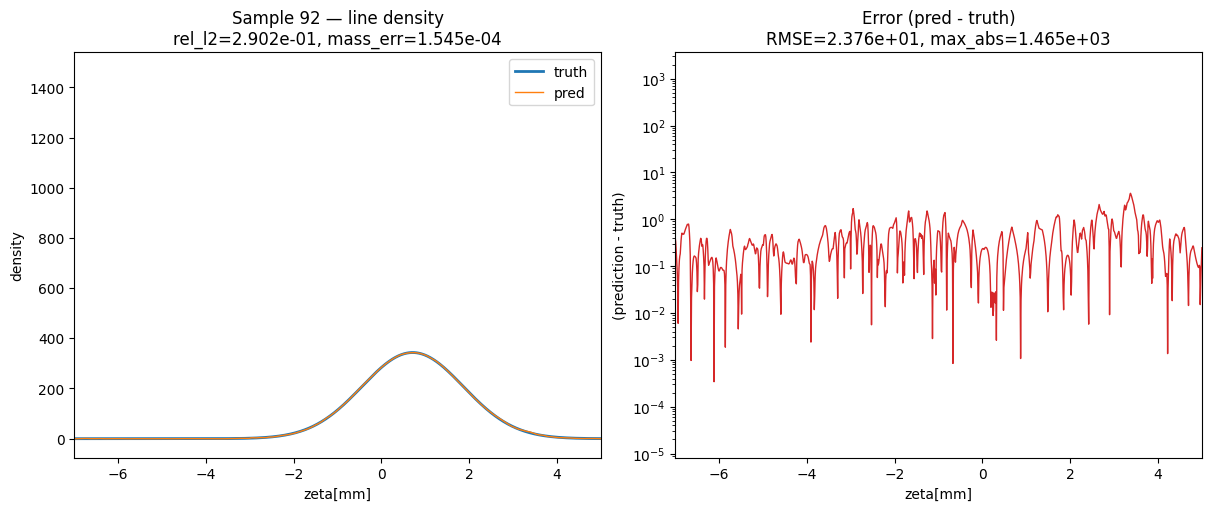
\includegraphics[width=\linewidth]{fno_longitudinal_reconstruction.png}\end{center}{\scriptsize Representative line-density prediction and residual. Qualitative validation on the FNO by working in reduced dimension.\par}
\end{column}
\end{columns}

\sources{\parencite{kovachki2023operators,desa2024pycolleff,zhou2023haissinski}.}

\end{frame}

% Original presentation frame 15
\begin{frame}[t,shrink=5]{A GNO represents lattice propagation as a learned kernel on a directed graph}
\begin{columns}[T,onlytextwidth]
\begin{column}{0.49\textwidth}
\begin{block}{Operator origin}
\[\mathcal K_\theta[v](x)=\int_D\kappa_\theta(x,y,\mu)v(y)\,\mathrm d\nu(y)\]
becomes, on graph nodes,
\[\mathcal K_\theta[v](x_i)\approx\sum_{j\in\mathcal N(i)}\omega_{ij}\kappa_\theta(x_i,x_j,\mu)v_j.\]
GNOs were introduced as graph-kernel neural operators for PDE solution maps and irregular domains.
\end{block}

\end{column}
\begin{column}{0.49\textwidth}
\begin{block}{GNO appears architecturally well-suited to accelerator propagation}
\begin{itemize}
\item Accelerator elements form an ordered, nonuniform sequence,
\item Directed edges enforce admissible upstream information transfer,
\item The learned kernel can use element type, position, relative geometry and global parameters,
\item Repeated local messages mirror composition of element-conditioned transformations.
\end{itemize}
\end{block}
{\scriptsize Prior accelerator latent-dynamics work conditions learned propagation on element descriptors. The present work tests a graph-kernel implementation for the FCC-ee HEB endpoint map.\par}
\end{column}
\end{columns}

\sources{\parencite{kovachki2023operators,li2020graph,wang2026latent}.}

\end{frame}

% Original presentation frame 16
\begin{frame}[t,shrink=5]{The selected CVAE–GNO checkpoint gives the lowest observed endpoint error and neural inference time}
\begin{columns}[T,onlytextwidth]
\begin{column}{0.49\textwidth}
\begin{block}{Residual graph-kernel update}
\[v_i^{\ell+1}=\sigma\left(Wv_i^\ell+\sum_{j\in\mathcal N(i)}K_\theta(h_i,h_j,\mu)v_j^\ell\right),\]
\[z_{i+1}=z_i+\Delta z_i.\]
The graph support is directed and local, the kernel is an effective latent interaction.
\end{block}
\begin{alertblock}{Selected checkpoint}
\[\epsilon_{\rm rel}=0.511,\quad\mathrm{SW}=0.014,\]\[\tau=2.338\ \mathrm{ms/sample}.\]
\end{alertblock}

\end{column}
\begin{column}{0.49\textwidth}
\begin{center}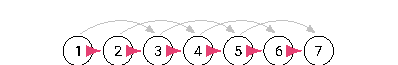
\includegraphics[width=\linewidth]{gno_directed_graph.pdf}\end{center}\begin{center}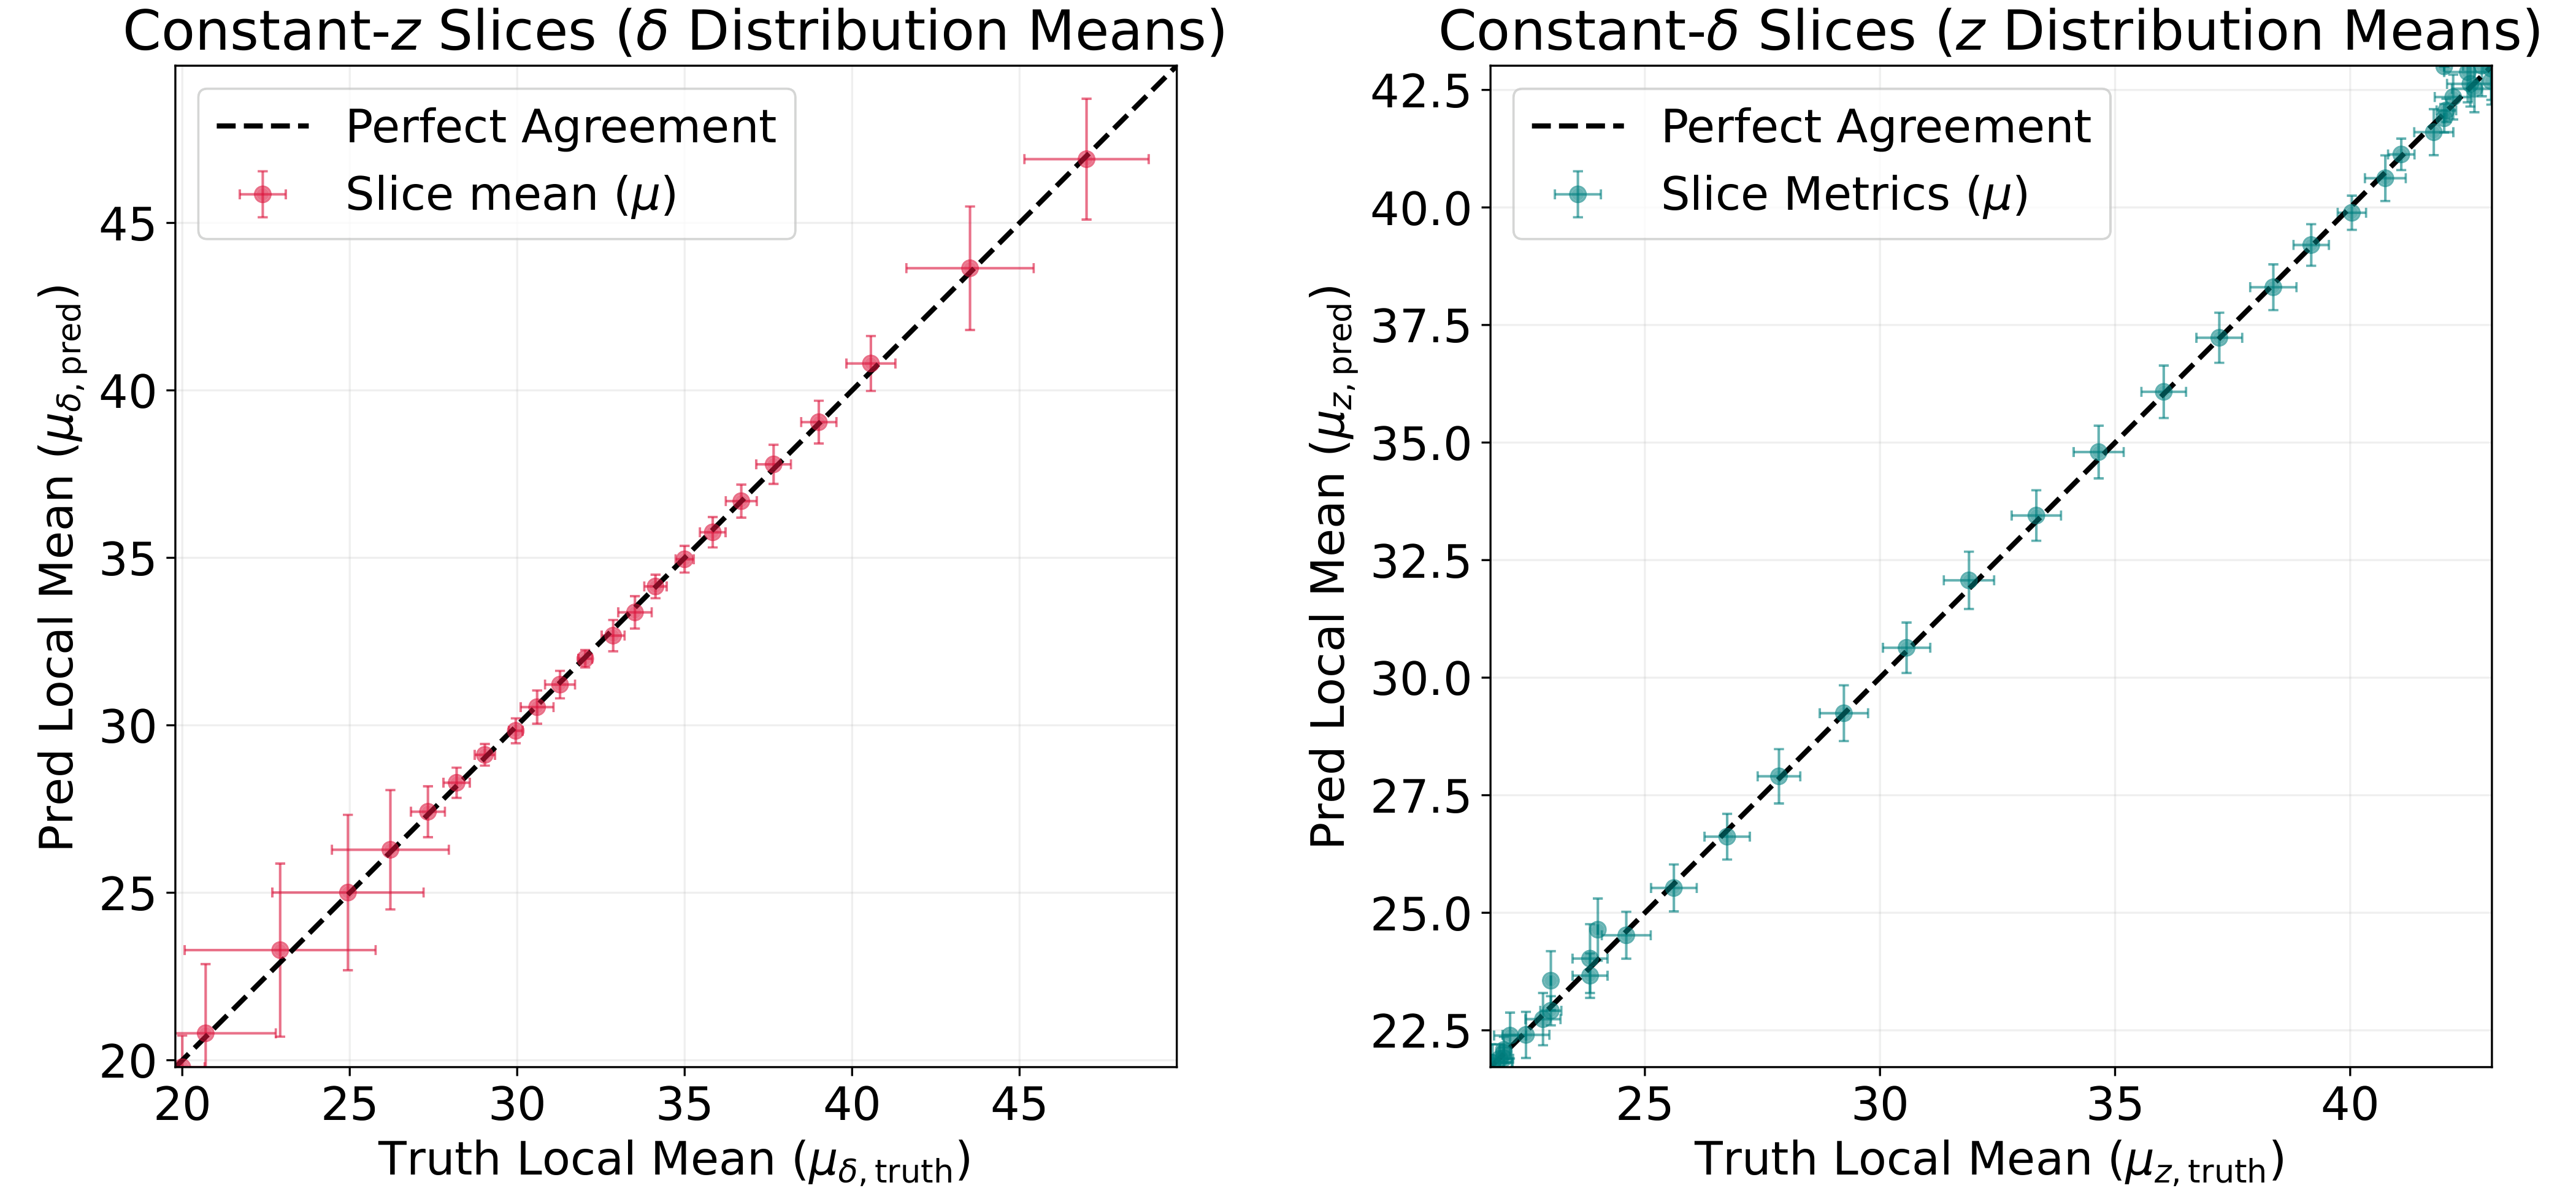
\includegraphics[width=\linewidth]{gno_longitudinal_slices.png}\end{center}{\scriptsize GNO conditional-slice consistency for the longitudinal marginal.\par}
\end{column}
\end{columns}

\sources{\parencite{kovachki2023operators,li2020graph}.}

\end{frame}

% Original presentation frame 17
\begin{frame}[t,shrink=5]{Windowed attention and GNO differ mainly in kernel parameterization and graph support}
\begin{columns}[T,onlytextwidth]
\begin{column}{0.49\textwidth}
\begin{block}{Common discrete operator}
\[(\mathcal T_\Theta h)_i=h_i+\sum_j A_{ij}K_\Theta(i,j,h_i,h_j,\mu)h_j.\]
\[A_{ij}^{\rm TF}=\mathbf1_{0\le i-j\le w},\quad A_{ij}^{\rm GNO}=\mathbf1_{j\in\mathcal N(i)}.\]
\end{block}
\begin{enumerate}
\item Windowed attention and GNO formalism are equivalent architecturally, but the kernels are parameterized differently.
\item The difference lies mainly in the support given to each one of the kernels in the transformation.
\end{enumerate}
\end{column}
\begin{column}{0.49\textwidth}
\begin{center}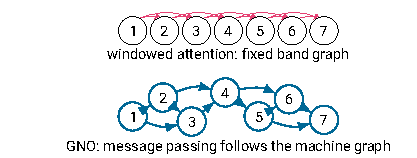
\includegraphics[width=\linewidth]{windowed_attention_and_gno_graphs.pdf}\end{center}\begin{block}{Depth composes local interactions}
After $L$ layers, local support can transmit information over multiple graph hops without direct all-to-all coupling.
\end{block}

\end{column}
\end{columns}

\sources{\parencite{li2020graph,vaswani2017attention}.}

\end{frame}

